\documentclass[aspectratio=169]{beamer}
\usetheme{Madrid}
\usecolortheme{default}

% Core packages only
\usepackage[utf8]{inputenc}
\usepackage[T1]{fontenc}
\usepackage{amsmath}
\usepackage{amsfonts}
\usepackage{amssymb}
\usepackage{graphicx}
\usepackage{xcolor}
\usepackage{booktabs}
\usepackage{tikz}
\usetikzlibrary{positioning,arrows.meta,shapes.geometric,fit}

% Graphics
\DeclareGraphicsExtensions{.pdf,.png,.jpg,.jpeg}

% Custom colors
\definecolor{juliagreen}{RGB}{56, 152, 38}
\definecolor{juliablue}{RGB}{64, 99, 216}
\definecolor{juliared}{RGB}{213, 99, 92}
\definecolor{juliapurple}{RGB}{149, 88, 178}
\definecolor{softgray}{RGB}{245,245,245}

% Beamer clean-up
\setbeamertemplate{navigation symbols}{}
\setbeamertemplate{footline}{}
\setbeamertemplate{page number in head/foot}{}

% Helpers
\newcommand{\tightlist}{\setlength{\itemsep}{4pt}\setlength{\parskip}{2pt}}

% Title page information
\title[IPA Framework]{The Information Propagation Framework}
\subtitle{A Julia toolkit for multi-metric analysis of DAG networks}
\author{}
\date{}

\begin{document}

\begin{frame}
\titlepage
\end{frame}


\begin{frame}{What is the IPA Framework?}
\begin{columns}[c]
\begin{column}{0.47\textwidth}
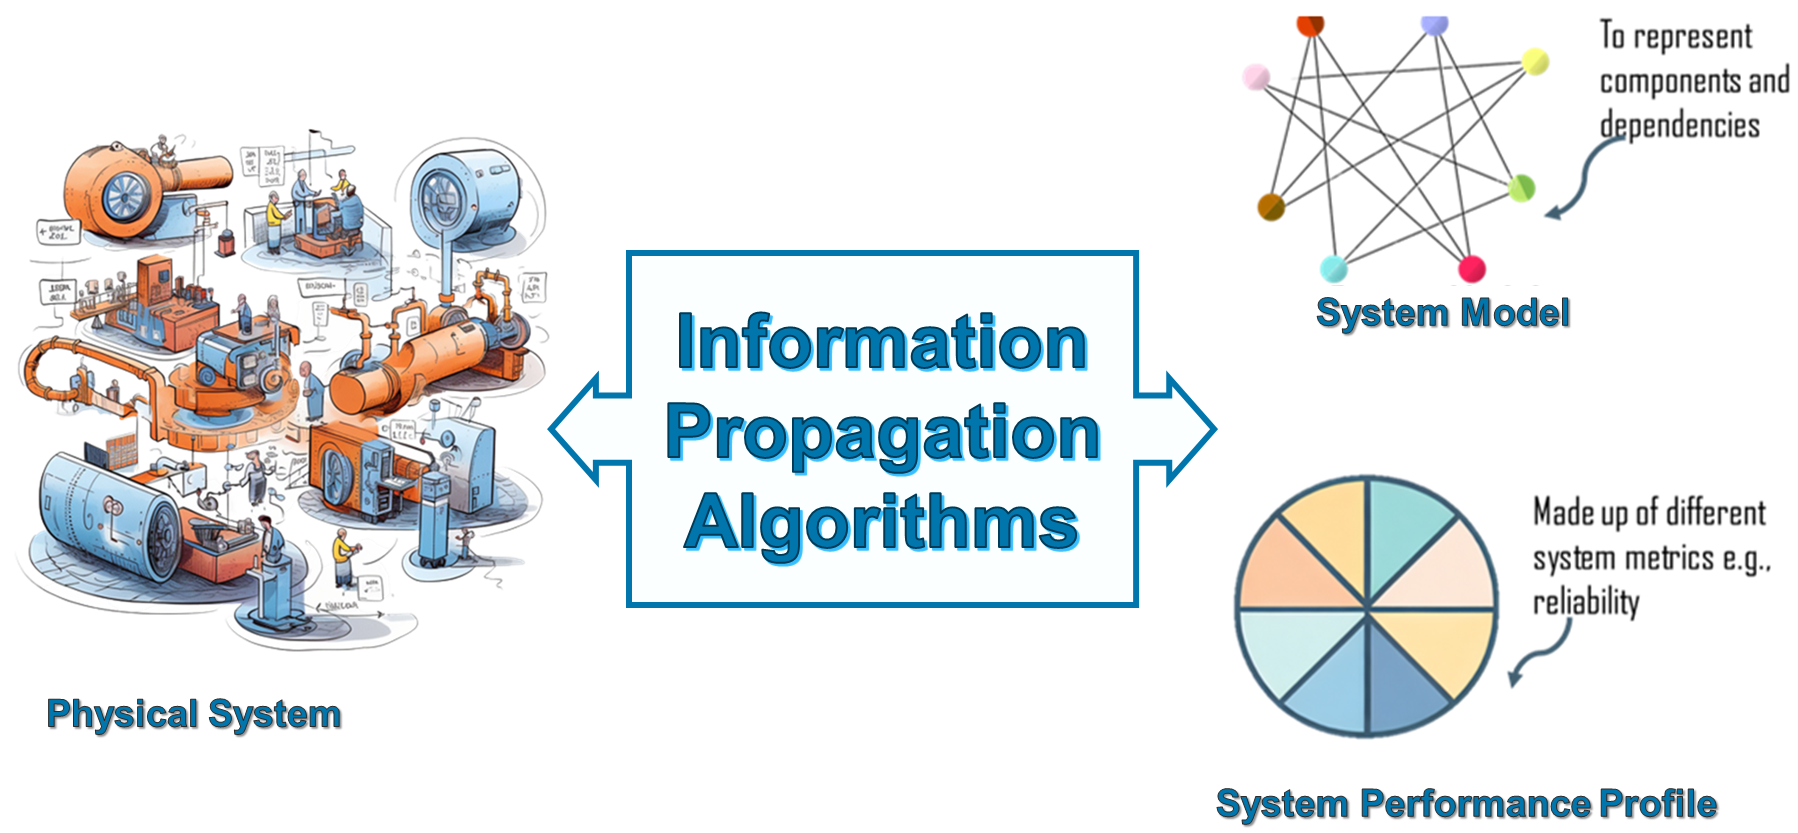
\includegraphics[width=\textwidth,height=0.68\textheight,keepaspectratio]{IPA.png}
\end{column}
\begin{column}{0.49\textwidth}
\begin{block}{In one sentence}
\small
IPA is a \textcolor{juliagreen}{\textbf{Julia-based}} framework for analysing how information, failure, time, cost, and capacity propagate through networks represented as directed acyclic graphs.
\end{block}

\vspace{0.2cm}
\begin{itemize}
\tightlist
\item One graph representation reused across multiple analyses
\item Exact DAG processing order from sources to sinks
\item Same framework supports reliability, flow, and scheduling questions
\end{itemize}
\end{column}
\end{columns}
\end{frame}


\begin{frame}{Core idea: process the DAG once, reuse everywhere}
\begin{columns}[c]
\begin{column}{0.52\textwidth}
\textbf{Two key ideas}
\begin{enumerate}
\tightlist
\item \textcolor{juliablue}{\textbf{Topological iteration sets}} give a safe processing order
\item \textcolor{juliagreen}{\textbf{Iterative message passing}} propagates values layer by layer
\end{enumerate}

\vspace{0.25cm}
\textbf{Benefits}
\begin{itemize}
\tightlist
\item No cyclic feedback issues
\item Dependencies resolved before downstream nodes
\item Natural parallelism within each layer
\item For most core analyses: $O(V+E)$ time on a DAG
\end{itemize}
\end{column}

\begin{column}{0.44\textwidth}
\begin{center}

\includegraphics[width=\textwidth,height=0.74\textheight,keepaspectratio]{msgpage.png}
\end{center}
\end{column}
\end{columns}
\end{frame}


\begin{frame}{Architecture and dependency chain}
\centering
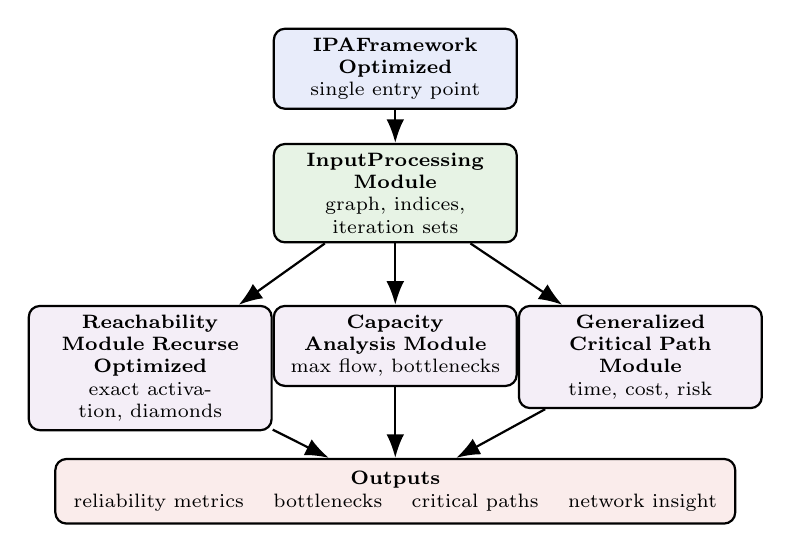
\begin{tikzpicture}[
    font=\scriptsize,
    node distance=0.42cm and 0.35cm,
    box/.style={rounded corners, draw, thick, align=center, minimum height=0.82cm, text width=2.85cm, fill=softgray},
    core/.style={box, fill=juliablue!12},
    prep/.style={box, fill=juliagreen!12},
    ana/.style={box, fill=juliapurple!10},
    resultbox/.style={box, fill=juliared!12},
    arr/.style={-{Latex[length=3mm]}, thick}
]

\node[core] (ipa) {\textbf{IPAFramework}\\\textbf{Optimized}\\single entry point};
\node[prep, below=of ipa] (input) {\textbf{InputProcessing}\\\textbf{Module}\\graph, indices, iteration sets};

\node[ana, below left=0.78cm and 0.0cm of input] (reach) {\textbf{Reachability}\\\textbf{Module Recurse}\\\textbf{Optimized}\\exact activation, diamonds};
\node[ana, below=0.78cm of input] (cap) {\textbf{Capacity}\\\textbf{Analysis Module}\\max flow, bottlenecks};
\node[ana, below right=0.78cm and 0.0cm of input] (crit) {\textbf{Generalized}\\\textbf{Critical Path}\\\textbf{Module}\\time, cost, risk};

\node[resultbox, below=0.9cm of cap, text width=8.4cm] (results) {\textbf{Outputs}\\reliability metrics \quad bottlenecks \quad critical paths \quad network insight};

\draw[arr] (ipa) -- (input);
\draw[arr] (input) -- (reach);
\draw[arr] (input) -- (cap);
\draw[arr] (input) -- (crit);
\draw[arr] (reach) -- (results);
\draw[arr] (cap) -- (results);
\draw[arr] (crit) -- (results);
\end{tikzpicture}

\vspace{0.1cm}
\scriptsize The structural work is done once in the input layer, then reused by the analysis modules.
\end{frame}


\begin{frame}{Input Processing layer: the shared graph object}
\begin{columns}[c]
\begin{column}{0.54\textwidth}
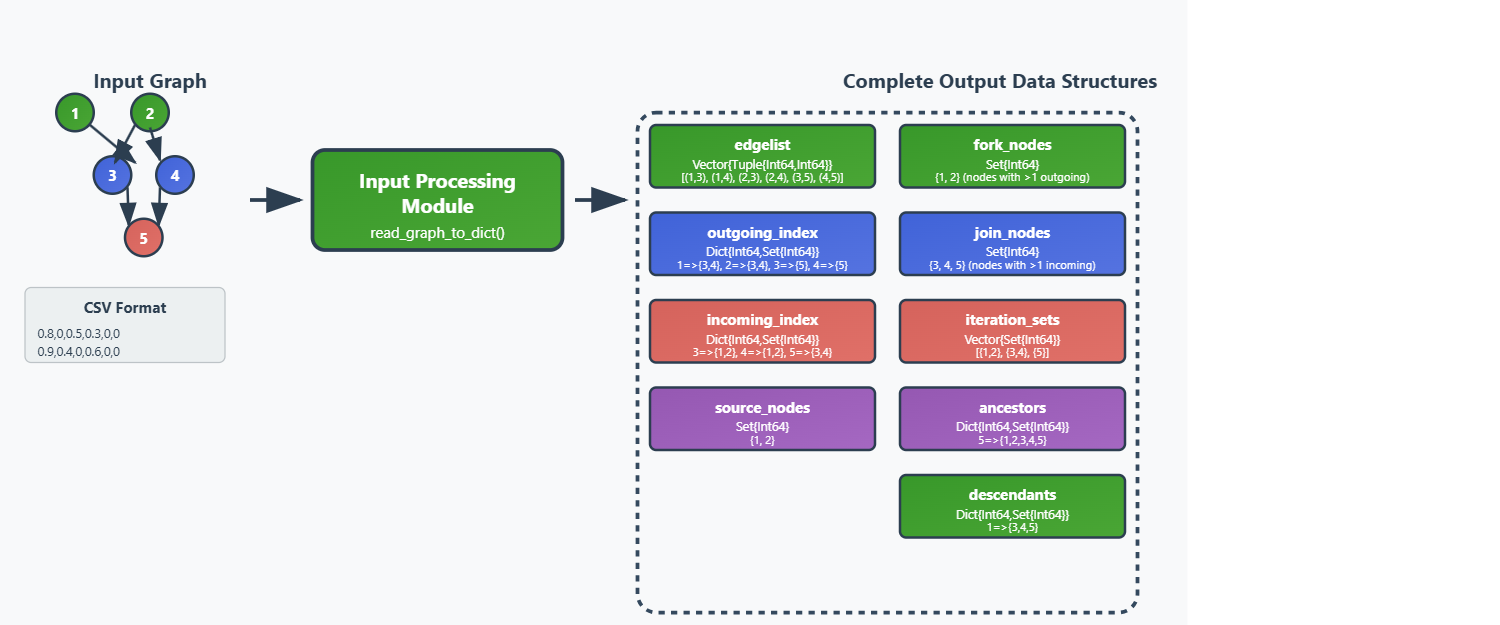
\includegraphics[width=\textwidth,height=0.76\textheight,keepaspectratio]{input_processing_outputs.png}
\end{column}
\begin{column}{0.42\textwidth}
\textbf{Computed once:}
\begin{itemize}
\tightlist
\item edge list
\item incoming / outgoing indices
\item source nodes
\item iteration sets
\item fork and join nodes
\item ancestors / descendants
\end{itemize}

\vspace{0.2cm}
\begin{block}{Why this matters}
\small
This turns later modules into \textbf{reusable analyses on one common DAG object}, instead of repeating graph preparation each time.
\end{block}
\end{column}
\end{columns}
\end{frame}


\begin{frame}{Reachability: what problem is it solving?}
\begin{columns}[c]
\begin{column}{0.56\textwidth}
\textbf{Goal}
\begin{itemize}
\tightlist
\item Compute the exact probability that a node becomes active
\item Activation means: \textbf{at least one causal path} from source nodes succeeds
\item Avoid double-counting when several paths overlap upstream
\end{itemize}

\vspace{0.25cm}
\textbf{Conceptually}
{\scriptsize
\[
P(v\ \text{active}) = P(\text{at least one active source-to-}v\text{ path})
\]
}

\vspace{0.15cm}
\begin{alertblock}{Main difficulty}
\small
The event is a \textbf{union of path events}, and those path events are often not independent.
\end{alertblock}
\end{column}

\begin{column}{0.38\textwidth}
\centering
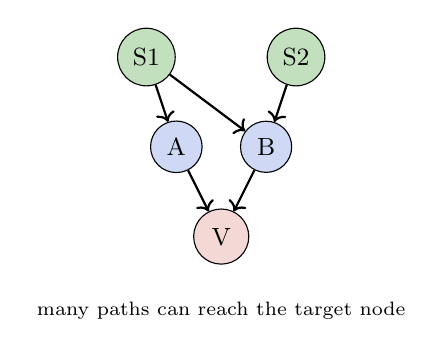
\begin{tikzpicture}[scale=0.95, font=\small]
\node[circle, draw, fill=juliagreen!30, minimum size=0.65cm] (s1) at (0,3) {S1};
\node[circle, draw, fill=juliagreen!30, minimum size=0.65cm] (s2) at (2,3) {S2};
\node[circle, draw, fill=juliablue!25, minimum size=0.65cm] (a) at (0.4,1.8) {A};
\node[circle, draw, fill=juliablue!25, minimum size=0.65cm] (b) at (1.6,1.8) {B};
\node[circle, draw, fill=juliared!25, minimum size=0.7cm] (t) at (1,0.6) {V};

\draw[->, thick] (s1) -- (a);
\draw[->, thick] (s1) -- (b);
\draw[->, thick] (s2) -- (b);
\draw[->, thick] (a) -- (t);
\draw[->, thick] (b) -- (t);

\node[below, align=center, font=\scriptsize] at (1,-0.15) {many paths can reach the\ target node};
\end{tikzpicture}
\end{column}
\end{columns}
\end{frame}


\begin{frame}{Reachability math: regular multi-parent cases}
\small
\begin{columns}[t]
\begin{column}{0.50\textwidth}
\begin{block}{Step 1: parent contributions}
For parent $i$ reaching child $j$ through edge $(i,j)$,
\[
P_{i\to j} = P(i)\,P(i\to j)
\]
\end{block}

\begin{block}{Step 2: combine multiple parents}
If parent-path events overlap, we need inclusion--exclusion:
\[
P(A\cup B)=P(A)+P(B)-P(A\cap B)
\]
\[
P\!\left(\bigcup_k A_k\right)\;\text{extends similarly}
\]
\end{block}
\end{column}

\begin{column}{0.47\textwidth}
\begin{block}{What the algorithm is really doing}
\begin{itemize}
\tightlist
\item Process nodes in topological order
\item Build activation from all upstream dependencies
\item Use exact combination rules when paths overlap
\end{itemize}
\end{block}

\vspace{0.15cm}
\begin{block}{Why not naive noisy-OR?}
\small
Noisy-OR is only safe when contributing events are independent. In DAGs with shared ancestry, that assumption can fail badly.
\end{block}
\end{column}
\end{columns}

\vspace{0.15cm}
\centering
\textcolor{juliapurple}{\textbf{So the core task is exact probability of a union of dependent path events.}}
\end{frame}


\begin{frame}{Reachability: the diamond problem}
\begin{columns}[c]
\begin{column}{0.52\textwidth}
\textbf{Diamond structure}
\begin{itemize}
\tightlist
\item A fork sends influence down multiple branches
\item Those branches reconverge later at a join
\item The branches are not independent because they share the same fork ancestry
\end{itemize}

\vspace{0.2cm}
\textbf{Why diamonds matter}
\begin{itemize}
\tightlist
\item They break naive independence assumptions
\item They are the main source of exact-conditioning work
\item They explain why local graph structure matters mathematically
\end{itemize}

\vspace{0.2cm}
\scriptsize
\[
P(\mathrm{join}) = \sum_{s \in \{0,1\}^{|F|}} P(\mathrm{join}\mid s)\,P(s)
\]
\end{column}

\begin{column}{0.43\textwidth}
\centering
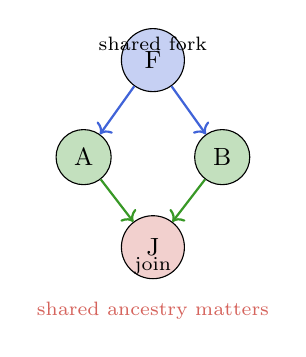
\begin{tikzpicture}[scale=0.88, font=\small]
\node[circle, draw, fill=juliablue!30, minimum size=0.8cm] (f) at (1.5,3.4) {F};
\node[circle, draw, fill=juliagreen!30, minimum size=0.7cm] (a) at (0.5,2.0) {A};
\node[circle, draw, fill=juliagreen!30, minimum size=0.7cm] (b) at (2.5,2.0) {B};
\node[circle, draw, fill=juliared!30, minimum size=0.8cm] (j) at (1.5,0.7) {J};

\draw[->, thick, juliablue] (f) -- (a);
\draw[->, thick, juliablue] (f) -- (b);
\draw[->, thick, juliagreen] (a) -- (j);
\draw[->, thick, juliagreen] (b) -- (j);

\node[above, font=\scriptsize] at (f) {shared fork};
\node[below, font=\scriptsize] at (j) {join};
\node[below, font=\scriptsize, text=juliared] at (1.5,0.05) {shared ancestry matters};
\end{tikzpicture}
\end{column}
\end{columns}
\end{frame}


\begin{frame}{Diamond decomposition: simplify the exact computation}
\begin{columns}[c]
\begin{column}{0.55\textwidth}
\textbf{Decomposition idea}
\begin{itemize}
\tightlist
\item Detect shared fork ancestry among parents of a join
\item Group parents into diamond-related subsystems
\item Extract only the local subgraph needed for exact conditioning
\end{itemize}

\vspace{0.3cm}
\textbf{Why decompose?}
\begin{itemize}
\tightlist
\item Simplifies reasoning inside complex DAGs
\item Keeps exact maths local to the problematic region
\item Makes nested diamond handling manageable
\item Gives a natural subsystem for recursion and parallel work
\end{itemize}
\end{column}

\begin{column}{0.45\textwidth}
\centering
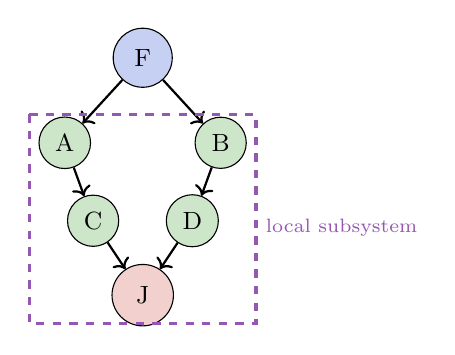
\begin{tikzpicture}[scale=0.9, font=\small]
\node[circle, draw, fill=juliablue!30, minimum size=0.75cm] (f) at (1.5,3.7) {F};
\node[circle, draw, fill=juliagreen!25, minimum size=0.65cm] (a) at (0.4,2.5) {A};
\node[circle, draw, fill=juliagreen!25, minimum size=0.65cm] (b) at (2.6,2.5) {B};
\node[circle, draw, fill=juliagreen!25, minimum size=0.65cm] (c) at (0.8,1.4) {C};
\node[circle, draw, fill=juliagreen!25, minimum size=0.65cm] (d) at (2.2,1.4) {D};
\node[circle, draw, fill=juliared!30, minimum size=0.78cm] (j) at (1.5,0.35) {J};

\draw[->, thick] (f) -- (a);
\draw[->, thick] (f) -- (b);
\draw[->, thick] (a) -- (c);
\draw[->, thick] (b) -- (d);
\draw[->, thick] (c) -- (j);
\draw[->, thick] (d) -- (j);

\draw[dashed, very thick, juliapurple] (-0.1,2.9) rectangle (3.1,-0.05);
\node[right, font=\scriptsize, text=juliapurple] at (3.1,1.3) {local subsystem};
\end{tikzpicture}

\end{column}
\end{columns}
\end{frame}


\begin{frame}{Reachability representations: same maths, different uncertainty models}
\begin{columns}[t]
\begin{column}{0.47\textwidth}
\textbf{Three exact representations}
\begin{itemize}
\tightlist
\item \textbf{Float:} one deterministic probability value
\item \textbf{Interval:} lower and upper probability bounds
\item \textbf{P-box:} richer uncertain probability description
\end{itemize}

\vspace{0.2cm}
\textbf{Typical inputs}
\begin{itemize}
\tightlist
\item node priors
\item edge probabilities
\item graph structure from input processing
\end{itemize}
\end{column}

\begin{column}{0.49\textwidth}
\textbf{Selection criteria}
\begin{itemize}
\tightlist
\item \textbf{Need speed?} use Float
\item \textbf{Need guaranteed bounds?} use Interval
\item \textbf{Need richer uncertainty?} use P-box
\item Trade-off is mainly between detail, memory, and runtime
\end{itemize}

\vspace{0.25cm}
\begin{block}{Key message}
\small
The reachability algorithmic logic is the same; what changes is the probability representation used by the arithmetic.
\end{block}
\end{column}
\end{columns}
\end{frame}


\begin{frame}{Capacity analysis: what is it solving?}
\begin{columns}[c]
\begin{column}{0.52\textwidth}
\textbf{Questions answered}
\begin{itemize}
\tightlist
\item What throughput can the network sustain?
\item Where is the bottleneck?
\item How do node and edge limits interact?
\item Which upgrades would most improve performance?
\end{itemize}

\vspace{0.2cm}
\begin{block}{Core view}
\small
Capacity analysis is about \textbf{how much can propagate}, not just whether something can propagate.
\end{block}
\end{column}

\begin{column}{0.42\textwidth}
\centering
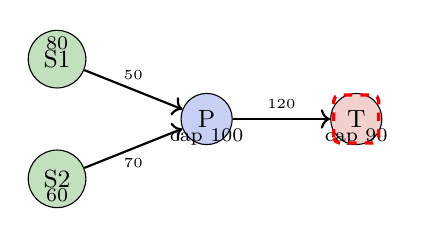
\begin{tikzpicture}[scale=0.95, font=\small]
\node[circle, draw, fill=juliagreen!30, minimum size=0.6cm] (s1) at (0,1.6) {S1};
\node[circle, draw, fill=juliagreen!30, minimum size=0.6cm] (s2) at (0,0) {S2};
\node[circle, draw, fill=juliablue!30, minimum size=0.65cm] (p) at (2,0.8) {P};
\node[circle, draw, fill=juliared!30, minimum size=0.65cm] (t) at (4,0.8) {T};

\draw[->, thick] (s1) -- (p) node[midway, above, font=\tiny] {50};
\draw[->, thick] (s2) -- (p) node[midway, below, font=\tiny] {70};
\draw[->, thick] (p) -- (t) node[midway, above, font=\tiny] {120};

\node[above, font=\scriptsize] at (s1) {80};
\node[below, font=\scriptsize] at (s2) {60};
\node[below, font=\scriptsize] at (p) {cap 100};
\node[below, font=\scriptsize] at (t) {cap 90};

\draw[red, very thick, dashed, rounded corners=2pt] (3.7,0.48) rectangle (4.3,1.12);
\end{tikzpicture}
\end{column}
\end{columns}
\end{frame}


\begin{frame}{Capacity analysis: maths, inputs, outputs, upgrades}
\small
\begin{columns}[t]
\begin{column}{0.50\textwidth}
\textbf{Core equation}
\[
\mathrm{Flow}[v] = \min\!\left(\sum_{u\in parents(v)} \min(\mathrm{Flow}[u], c_{uv}),\; c_v\right)
\]

\textbf{Inputs}
\begin{itemize}
\tightlist
\item node capacities
\item edge capacities
\item source input rates
\item target nodes
\end{itemize}
\end{column}

\begin{column}{0.46\textwidth}
\textbf{Outputs}
\begin{itemize}
\tightlist
\item total max flow
\item bottleneck report
\item path analysis / validation
\item comparative or uncertain variants
\end{itemize}

\vspace{0.15cm}
\begin{block}{Upgrade idea}
\small
Because the module identifies constrained edges and nodes, it can support upgrade recommendations such as \textbf{which component increase gives the biggest throughput gain}.
\end{block}
\end{column}
\end{columns}
\end{frame}


\begin{frame}{Critical path analysis: what is it solving?}
\begin{columns}[c]
\begin{column}{0.53\textwidth}
\textbf{Questions answered}
\begin{itemize}
\tightlist
\item What is the longest or critical path?
\item What is the earliest completion time?
\item What is the maximum accumulated cost or risk?
\item Which nodes or edges dominate the result?
\end{itemize}

\vspace{0.2cm}
\begin{block}{Key idea}
\small
This is not restricted to time. The same pattern works for cost, risk, and other path-based metrics.
\end{block}
\end{column}

\begin{column}{0.41\textwidth}
\centering
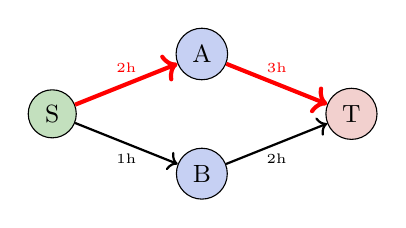
\begin{tikzpicture}[scale=0.95, font=\small]
\node[circle, draw, fill=juliagreen!30, minimum size=0.6cm] (s) at (0,0) {S};
\node[circle, draw, fill=juliablue!30, minimum size=0.6cm] (a) at (2,0.8) {A};
\node[circle, draw, fill=juliablue!30, minimum size=0.6cm] (b) at (2,-0.8) {B};
\node[circle, draw, fill=juliared!30, minimum size=0.6cm] (t) at (4,0) {T};

\draw[->, thick, red, line width=1.5pt] (s) -- (a) node[midway, above, font=\tiny] {2h};
\draw[->, thick] (s) -- (b) node[midway, below, font=\tiny] {1h};
\draw[->, thick, red, line width=1.5pt] (a) -- (t) node[midway, above, font=\tiny] {3h};
\draw[->, thick] (b) -- (t) node[midway, below, font=\tiny] {2h};
\end{tikzpicture}
\end{column}
\end{columns}
\end{frame}


\begin{frame}{Critical path maths: a generalized three-stage engine}
\small
\textbf{For each node in topological order:}
\begin{align*}
\text{Stage 1: } &\mathrm{Propagate}(\text{parent value},\text{ edge value}) \\
\text{Stage 2: } &\mathrm{Combine}(\text{all propagated parent values}) \\
\text{Stage 3: } &\mathrm{NodeFn}(\text{combined input},\text{ node value})
\end{align*}

\vspace{0.2cm}
\begin{center}
\begin{tabular}{|l|c|c|c|}
\hline
\textbf{Analysis} & \textbf{Combine} & \textbf{Propagate} & \textbf{NodeFn} \\
\hline
Time & $\max$ & $parent + edge$ & $input + duration$ \\
Cost & $\max$ & $parent + edge$ & $input + cost$ \\
Bottleneck & $\max$ & $\min(parent,edge)$ & $\min(input,cap)$ \\
Risk & $\max$ & $parent + edge$ & $input + risk$ \\
\hline
\end{tabular}
\end{center}

\vspace{0.15cm}
\centering
\textcolor{juliablue}{\textbf{One generalized engine, many path-based analyses.}}
\end{frame}


\begin{frame}{Critical path inputs, outputs, and extensibility}
\begin{columns}[t]
\begin{column}{0.48\textwidth}
\textbf{Typical inputs}
\begin{itemize}
\tightlist
\item node durations / costs / risks
\item edge delays / transition costs
\item project start value
\item chosen combination, propagation, and node functions
\end{itemize}

\vspace{0.2cm}
\textbf{Outputs}
\begin{itemize}
\tightlist
\item critical value at target nodes
\item critical path nodes
\item backward-pass or slack-style analysis
\end{itemize}
\end{column}

\begin{column}{0.48\textwidth}
\begin{block}{Why it is useful in the framework}
\small
It reuses the same DAG preprocessing and lets the user swap in different semantics without changing the graph logic.
\end{block}

\vspace{0.15cm}
\begin{block}{Extension idea}
\small
Any metric with a sensible path propagation rule can be inserted here: time, cost, risk, resilience score, or a custom domain-specific quantity.
\end{block}
\end{column}
\end{columns}
\end{frame}


\begin{frame}{Framework summary}
\begin{columns}[c]
\begin{column}{0.41\textwidth}
\vspace{0.25cm}
\begin{block}{Best fit}
\small
Projects where the network is fixed but the question changes: reliability, throughput, timing, cost, or resilience.
\end{block}

\vspace{0.15cm}
\textcolor{juliagreen}{\textbf{In short:}} preprocess once, analyse many times.
\end{column}

\begin{column}{0.55\textwidth}
\begin{center}
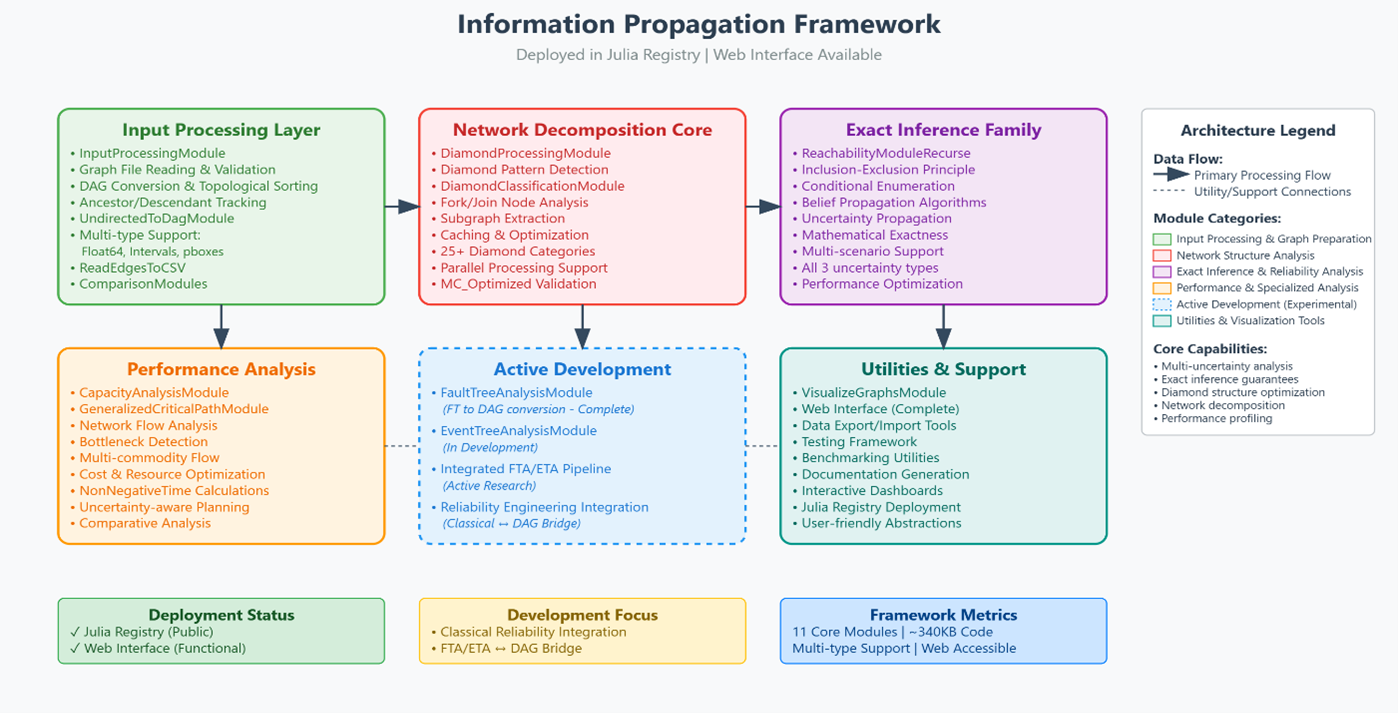
\includegraphics[width=\textwidth,height=0.78\textheight,keepaspectratio]{IPa-FULLPICTURE.png}
\end{center}
\end{column}
\end{columns}
\end{frame}


\begin{frame}
\centering
\Huge Thank you

\vspace{0.4cm}
\Large Questions?
\end{frame}

\end{document}